\documentclass[11pt,oneside]{article}

\usepackage[T1]{fontenc}
\usepackage[utf8]{inputenc}
\usepackage{lmodern}
\usepackage[margin=1.05in]{geometry}
\usepackage{microtype}
\usepackage{amsmath,amssymb,amsthm,mathtools}
\usepackage{bm}
\usepackage{booktabs,longtable,array,tabularx}
\usepackage{enumitem}
\usepackage{xcolor}
\usepackage{graphicx}
\usepackage{tikz}
\usetikzlibrary{arrows.meta,positioning,shapes.geometric,calc}
\usepackage{listings}
\usepackage{fancyhdr}
\usepackage{hyperref}
\usepackage{bookmark}

\definecolor{deepblue}{RGB}{24,63,112}
\definecolor{deepred}{RGB}{132,35,35}
\definecolor{deepgreen}{RGB}{27,105,67}
\definecolor{softgray}{RGB}{245,246,248}
\definecolor{midgray}{RGB}{88,94,105}

\hypersetup{
  colorlinks=true,
  linkcolor=deepblue,
  citecolor=deepgreen,
  urlcolor=deepblue,
  pdftitle={New Structural Progress on the Alaoglu--Erdos Conjecture},
  pdfauthor={OpenAI GPT-5.6 Pro},
  pdfsubject={Transcendence theory, periods, and exponential Diophantine equations}
}

\pagestyle{fancy}
\fancyhf{}
\fancyhead[L]{Alaoglu--Erd\H{o}s progress report}
\fancyhead[R]{22 August 2026}
\fancyfoot[C]{\thepage}
\setlength{\headheight}{14pt}

\setlist[itemize]{leftmargin=1.6em,itemsep=0.25em,topsep=0.4em}
\setlist[enumerate]{leftmargin=1.8em,itemsep=0.3em,topsep=0.4em}

\newtheorem{theorem}{Theorem}[section]
\newtheorem{proposition}[theorem]{Proposition}
\newtheorem{lemma}[theorem]{Lemma}
\newtheorem{corollary}[theorem]{Corollary}
\newtheorem{conjecture}[theorem]{Conjecture}
\newtheorem{question}[theorem]{Question}
\theoremstyle{definition}
\newtheorem{definition}[theorem]{Definition}
\newtheorem{remark}[theorem]{Remark}
\newtheorem{program}[theorem]{Research program}

\newcommand{\N}{\mathbb N}
\newcommand{\Z}{\mathbb Z}
\newcommand{\Q}{\mathbb Q}
\newcommand{\R}{\mathbb R}
\newcommand{\C}{\mathbb C}
\newcommand{\Qbar}{\overline{\mathbb Q}}
\newcommand{\rad}{\operatorname{rad}}
\newcommand{\ord}{\operatorname{ord}}
\newcommand{\rank}{\operatorname{rank}}
\newcommand{\Span}{\operatorname{span}}
\newcommand{\per}{\operatorname{per}}
\newcommand{\supp}{\operatorname{supp}}
\newcommand{\Espace}{\mathscr E_{2,3}}
\newcommand{\Ispace}{\mathscr I_{2,3}}
\newcommand{\vp}[1]{v_{#1}}
\newcommand{\Li}{\operatorname{Li}}
\newcommand{\dd}{\,\mathrm d}

\newenvironment{statusbox}[1]{%
  \begin{center}\begin{minipage}{0.94\textwidth}
  \colorbox{softgray}{\parbox{0.965\textwidth}{\textbf{#1}\par\smallskip}}
  \vspace{-0.8em}\begin{quote}\small
}{\end{quote}\end{minipage}\end{center}}

\lstset{
  basicstyle=\ttfamily\small,
  backgroundcolor=\color{softgray},
  frame=single,
  rulecolor=\color{midgray},
  breaklines=true,
  columns=fullflexible,
  showstringspaces=false
}

\title{\textbf{New Structural Progress on the Alaoglu--Erd\H{o}s Conjecture}\\[0.4em]
\large A canonical-generator dichotomy, a sparse weight-two period obstruction,\\
and radical-full continued-fraction gaps}
\author{Research progress report prepared by OpenAI GPT-5.6 Pro}
\date{22 August 2026}

\begin{document}
\maketitle

\begin{abstract}
The Alaoglu--Erd\H{o}s conjecture asks whether
\[
  2^x,3^x\in\Z \quad\Longrightarrow\quad x\in\Z
\]
for real $x$.  This document is a non-redundant supplement to the supplied unified report.  It does not repeat that report's broad survey of determinant, interpolation, Kummer, $K$-theoretic, Chebotarev, dynamical, information-theoretic, and general analytic approaches.  Instead it develops three new, sharply delimited pieces of progress.

First, the proved Six Exponentials Theorem, combined with an elementary saturation argument for prime-valuation lattices, gives a strong dichotomy.  Either the solution set is exactly $\N_0$, or there is a \emph{unique} shift-normalized, perfect-power-primitive transcendental solution $\xi$ and every solution is
\[
  r+s\xi\qquad(r,s\in\N_0).
\]
Consequently, one extra integer point on $Y=X^{\log 3/\log 2}$ forces a full two-dimensional semigroup of points and changes the counting function from order $\log H$ to an explicit positive multiple of $(\log H)^2$.  This yields an exact counting reformulation of the conjecture.

Second, a putative counterexample defines a sparse nonzero quadratic Kummer class
\[
  \mathcal F_{m,n}=L(m)L_3-L(n)L_2
\]
whose real period is zero.  Every counterexample necessarily contains a prime $q\notin\{2,3\}$, and the $q$-contraction of this class is the explicit nonzero logarithm
\[
  a_q\log 3-b_q\log 2=\log\!\left(3^{a_q}/2^{b_q}\right).
\]
The same prime gives a nonzero mixed valuation--$q$-adic-logarithm realization.  Thus a counterexample would be not merely an unspecified failure of a period conjecture, but a zero archimedean period with a finite, quantitatively nonzero first coaction descendant.

Third, assuming the $abc$ conjecture, the coprime gaps obtained by comparing the non-base part of $m^q$ with a nearby power of $2$ (and similarly for $n^q$ and $3$) are asymptotically radical-full:
\[
  \frac{\log\rad |G_j|}{\log |G_j|}\longrightarrow 1.
\]
This gives a rigorous obstruction to a naive Frey-curve strategy based on the repeated powers in the two main terms: the gap itself supplies exponentially large new radical.

No unconditional proof of the Alaoglu--Erd\H{o}s conjecture is claimed.  The principal value of the report is to replace several diffuse goals by exact theorems, a canonical counterexample normal form, and two narrowly targeted missing principles that can be attacked independently or formalized in Lean.
\end{abstract}

\tableofcontents
\newpage

\section{Executive assessment}

\subsection{What is genuinely new here}

The supplied report already catalogues a very wide range of attacks.  Repeating those ideas with different notation would not constitute progress.  The present supplement therefore concentrates on the following results and reductions.

\begin{longtable}{>{\raggedright\arraybackslash}p{0.26\textwidth} >{\raggedright\arraybackslash}p{0.22\textwidth} >{\raggedright\arraybackslash}p{0.42\textwidth}}
\toprule
Contribution & Status & Mathematical content\\
\midrule
\endfirsthead
\toprule
Contribution & Status & Mathematical content\\
\midrule
\endhead
Canonical-generator dichotomy & Unconditional, using the proved Six Exponentials Theorem & If any nonintegral solution exists, there is a unique normalized primitive generator $\xi$, and all solutions are $r+s\xi$ with $r,s\ge 0$.\\
\addlinespace
Sharp counting reformulation & Unconditional consequence of the dichotomy & Integer points on $Y=X^{\log3/\log2}$ have either linear or quadratic logarithmic growth; any $o((\log H)^2)$ upper bound proves the conjecture.\\
\addlinespace
Sparse quadratic-period certificate & Unconditional formal algebra plus standard mixed-Tate interpretation & A counterexample gives a nonzero weight-two Kummer class with zero real period and an explicit nonzero prime contraction.\\
\addlinespace
Archimedean/$q$-adic mismatch & Unconditional local calculation & At an external prime $q$, the mixed valuation--logarithm realization is $\log_q(3^{a_q}/2^{b_q})\ne0$.\\
\addlinespace
Radical-full gap theorem & Conditional on $abc$ & Reduced convergent gaps have radical asymptotic to their full size on a logarithmic scale.\\
\addlinespace
Frey-level audit & Conditional interpretation & Repeated powers in the main terms do not lead to a bounded radical: the gap injects exponentially many prime bits.\\
\addlinespace
Formalization architecture & Rigorous dependency separation & The elementary algebra can be formalized now; Six Exponentials, Gelfond--Schneider, the period principle, and $abc$ can be isolated as named interfaces.\\
\bottomrule
\end{longtable}

\begin{statusbox}{Status discipline}
Every statement below is labeled as proved, conditional, or programmatic.  In particular, the motivic discussion is used to identify a precise missing injectivity statement; it is not presented as though the period conjecture were already known.  Reports about work by other systems are not used as mathematical evidence.
\end{statusbox}

\subsection{The central new picture}

Write
\[
  \Ispace=\{t\in\R_{\ge0}:2^t,3^t\in\Z\}.
\]
The new structural theorem says that there are only two possible global shapes:
\[
  \Ispace=\N_0,
  \qquad\text{or}\qquad
  \Ispace=\N_0+\N_0\xi
\]
for one canonical transcendental $\xi$.  In the second case, if
\[
  M=2^\xi,\qquad N=3^\xi,
\]
then every point is
\[
  (2^t,3^t)=(2^rM^s,3^rN^s),\qquad r,s\in\N_0.
\]
At the same time, all of those points carry only scalar multiples of one quadratic period obstruction.  Thus a counterexample would create many integer points but only one primitive weight-two relation.  This explains both the promise and the limitation of counting and determinant methods: the geometric data proliferate quadratically, while the period relation itself remains rank one.

\section{Basic reductions and a canonical normal form}

Throughout, suppose
\[
  m=2^x\in\Z_{>0},\qquad n=3^x\in\Z_{>0}.
\]
We use
\[
  a_p=v_p(m),\qquad b_p=v_p(n).
\]
Only finitely many $a_p,b_p$ are nonzero.

\subsection{Rational and algebraic exponents}

\begin{lemma}[Rational exponents]
If $x\in\Q$ and $2^x\in\Z$, then $x\in\Z$.
\end{lemma}

\begin{proof}
Write $x=A/D$ with $D>0$ and $\gcd(A,D)=1$.  Since $2^x$ is a positive integer $m$,
\[
  m^D=2^A.
\]
Unique factorization gives $D v_2(m)=A$, so $D\mid A$.  Hence $D=1$.
\end{proof}

\begin{corollary}
A nonintegral solution $x$ is irrational.
\end{corollary}

\begin{lemma}[Gelfond--Schneider reduction]
A nonintegral solution $x$ is transcendental.
\end{lemma}

\begin{proof}
If $x$ were algebraic and irrational, the Gelfond--Schneider theorem would make every value of $2^x$ transcendental.  The positive real value is $m\in\Z$, a contradiction.
\end{proof}

\begin{lemma}
The two numbers $\log 2/\log 3$ and $\log 3/\log 2$ are transcendental.
\end{lemma}

\begin{proof}
The ratio $\log 2/\log 3$ is not rational, since a rational relation would give $2^u=3^v$ for nonzero integers $u,v$.  If the ratio were algebraic irrational, then
\[
  3^{\log2/\log3}=2
\]
would contradict Gelfond--Schneider.  Its reciprocal is therefore transcendental as well.
\end{proof}

\subsection{An external prime is unavoidable}

\begin{proposition}[Support escape]
If $m=2^x$ and $n=3^x$ are integers and every prime divisor of $mn$ belongs to $\{2,3\}$, then $x\in\Z$.
\end{proposition}

\begin{proof}
Write
\[
  m=2^a3^c,\qquad n=2^b3^d
\]
with $a,b,c,d\in\N_0$.  Put $r=\log2/\log3$.  The equality
\[
  \log m\,\log3-\log n\,\log2=0
\]
becomes
\[
  c+(a-d)r-br^2=0.
\]
Since $r$ is transcendental, all three rational coefficients vanish.  Thus $b=c=0$ and $a=d$.  Hence $m=2^a$, $n=3^a$, and $x=a$.
\end{proof}

\begin{corollary}[External-prime lemma]
Every nonintegral solution has a prime divisor $q\notin\{2,3\}$ of $mn$.
\end{corollary}

This elementary fact is the hinge for the coaction and $q$-adic certificates later in the report.

\subsection{Shift normalization and perfect-power primitivity}

There are two elementary operations on a solution.

\paragraph{Diagonal shift.}
Let
\[
  k=\min\{a_2,b_3\}.
\]
Since $2^{a_2}\le m=2^x$ and $3^{b_3}\le n=3^x$, one has $k\le x$.  Define
\[
  x_1=x-k,\qquad m_1=m/2^k,\qquad n_1=n/3^k.
\]
Then
\[
  2^{x_1}=m_1,\qquad 3^{x_1}=n_1,
\]
and
\[
  \min\{v_2(m_1),v_3(n_1)\}=0.
\]
If $x$ is nonintegral, then $x_1>0$ and is nonintegral.

\paragraph{Common-root descent.}
Let
\[
 d=\gcd\bigl(\{v_p(m_1):p\text{ prime}\}\cup
              \{v_p(n_1):p\text{ prime}\}\bigr).
\]
Then $m_1=M^d$ and $n_1=N^d$ for positive integers $M,N$.  Put
\[
  \xi=\frac{x_1}{d}.
\]
The positive real roots give
\[
  2^\xi=M,
  \qquad
  3^\xi=N.
\]
Moreover,
\[
 \min\{v_2(M),v_3(N)\}=0,
 \qquad
 \gcd\bigl(\{v_p(M)\}_p\cup\{v_p(N)\}_p\bigr)=1.
\]
If $x$ was nonintegral, then $\xi$ is nonintegral, for otherwise $x=k+d\xi$ would be an integer.

\begin{definition}[Normalized primitive solution]
A nonintegral solution $\xi$ with $M=2^\xi$ and $N=3^\xi$ is \emph{normalized primitive} if
\[
  \min\{v_2(M),v_3(N)\}=0
\]
and the gcd of all prime exponents occurring in $M$ and $N$ is $1$.
\end{definition}

\begin{proposition}[Canonical reduction]
Every nonintegral solution produces a normalized primitive solution by a finite, explicit shift-and-root operation.
\end{proposition}

\section{The Six Exponentials plane}

\subsection{The algebraic-exponent space}

Define
\[
  \Espace=\{z\in\C:2^z,3^z\in\Qbar^\times\},
\]
where $2^z=e^{z\log2}$ and $3^z=e^{z\log3}$ use the positive real logarithms of $2$ and $3$.

\begin{lemma}
The set $\Espace$ is a vector space over $\Q$.
\end{lemma}

\begin{proof}
It is closed under addition and subtraction because algebraic numbers are closed under multiplication and division.  If $z\in\Espace$ and $D\ge1$, then $2^{z/D}$ is a root of $T^D-2^z$ and $3^{z/D}$ is a root of $T^D-3^z$, hence both are algebraic.  This gives closure under rational scalar multiplication.
\end{proof}

\begin{theorem}[Six Exponentials consequence]
One has
\[
  \dim_{\Q}\Espace\le2.
\]
\end{theorem}

\begin{proof}
The numbers $\log2$ and $\log3$ are linearly independent over $\Q$.  If $z_1,z_2,z_3\in\Espace$ were linearly independent over $\Q$, all six numbers
\[
 e^{z_j\log2},\quad e^{z_j\log3}\qquad(1\le j\le3)
\]
would be algebraic, contradicting the Six Exponentials Theorem.
\end{proof}

\begin{corollary}[Exceptional plane]
If a nonintegral solution $x$ exists, then
\[
  \Espace=\Q+\Q x.
\]
\end{corollary}

\begin{proof}
Both $1$ and $x$ lie in $\Espace$, and they are linearly independent over $\Q$.  The preceding theorem leaves no room for a third direction.
\end{proof}

This observation is standard in spirit, but its combination with the valuation-saturation argument below produces a much stronger classification than the usual statement that the conjecture is a special case of Four Exponentials.

\subsection{Immediate transcendence consequences}

\begin{corollary}
Assume $x$ is a nonintegral solution.  If $z\notin\Q+\Q x$, then at least one of $2^z,3^z$ is transcendental.
\end{corollary}

\begin{corollary}[Transcendence one level higher]
For a nonintegral solution $x$, at least one of
\[
  m^x=2^{x^2},\qquad n^x=3^{x^2}
\]
is transcendental.
\end{corollary}

\begin{proof}
Since $x$ is transcendental, the three numbers $1,x,x^2$ are linearly independent over $\Q$.  Hence $x^2\notin\Espace$.
\end{proof}

\begin{corollary}
For every polynomial $P\in\Q[T]$ of degree at least $2$, at least one of $2^{P(x)}$ and $3^{P(x)}$ is transcendental.
\end{corollary}

The last statements identify a concrete completion strategy: it would suffice to derive, from integrality of $m$ and $n$, the algebraicity of both $2^{P(x)}$ and $3^{P(x)}$ for a single nonlinear rational polynomial $P$.

\section{Prime-valuation saturation and the canonical-generator theorem}

Let $\xi$ be a normalized primitive solution, and put
\[
 M=2^\xi,\qquad N=3^\xi,
\]
with
\[
 a_p=v_p(M),\qquad b_p=v_p(N).
\]
Thus
\[
 \min\{a_2,b_3\}=0,
 \qquad
 \gcd(\{a_p\}_p\cup\{b_p\}_p)=1.
\]
By the external-prime lemma, at least one $a_q$ or $b_q$ is positive for some $q\notin\{2,3\}$.

\subsection{The valuation lattice}

Every $y\in\Espace$ has a unique expression
\[
  y=r+s\xi,
  \qquad r,s\in\Q,
\]
because $1,\xi$ are linearly independent over $\Q$.  The integrality of $2^y$ and $3^y$ is controlled by the linear forms
\[
  r\delta_{p,2}+s a_p,
  \qquad
  r\delta_{p,3}+s b_p.
\]

\begin{proposition}[Valuation criterion]
Let $y=r+s\xi$ with $r,s\in\Q$.  Then $y\in\Ispace$ if and only if, for every prime $p$,
\[
 r\delta_{p,2}+s a_p\in\N_0,
 \qquad
 r\delta_{p,3}+s b_p\in\N_0.
\]
\end{proposition}

\begin{proof}
Choose $D>0$ with $Dr,Ds\in\Z$.  If $2^y=A\in\Z_{>0}$, then
\[
 A^D=2^{Dr}M^{Ds},
\]
and taking $p$-adic valuations gives the first family of conditions.  The same argument gives the second family.  Conversely, if all displayed exponents are nonnegative integers, unique factorization reconstructs positive integers whose $D$th powers are $2^{Dr}M^{Ds}$ and $3^{Dr}N^{Ds}$; uniqueness of positive real $D$th roots gives $2^y$ and $3^y$ themselves.
\end{proof}

One may package the integrality conditions in an integer matrix whose rows are
\[
 (1,a_2),\quad (0,a_p)\ (p\ne2),\quad
 (1,b_3),\quad (0,b_p)\ (p\ne3).
\]
The gcd of its $2\times2$ minors is
\begin{equation}\label{eq:saturation-index}
 \Delta=
 \gcd\Bigl(
   b_3-a_2,
   \{a_p:p\ne2\},
   \{b_p:p\ne3\}
 \Bigr).
\end{equation}
For a shift-normalized pair, this is exactly the gcd of all prime exponents of $M$ and $N$.  Thus primitivity says $\Delta=1$: the valuation lattice is saturated.

\subsection{An elementary denominator-elimination proof}

The following proof is designed to be easy to formalize and avoids invoking Smith normal form.

\begin{theorem}[Saturation theorem]
For a normalized primitive solution $\xi$, every $y\in\Ispace$ has a unique representation
\[
  y=A+B\xi
\]
with $A,B\in\N_0$.
\end{theorem}

\begin{proof}
By the exceptional-plane corollary, write
\[
 y=\frac{A+B\xi}{D}
\]
with $A,B,D\in\Z$, $D>0$, and $\gcd(A,B,D)=1$.
Let
\[
 c_p=v_p(2^y),\qquad d_p=v_p(3^y).
\]
The valuation criterion gives
\begin{align}
 D c_p&=A\delta_{p,2}+B a_p,\label{eq:val1}\\
 D d_p&=A\delta_{p,3}+B b_p.\label{eq:val2}
\end{align}
For $p\ne2$, equation \eqref{eq:val1} gives $D\mid B a_p$.  For $p\ne3$, equation \eqref{eq:val2} gives $D\mid B b_p$.  The special equations at $p=2$ and $p=3$ imply
\[
 D\mid A+B a_2,
 \qquad
 D\mid A+B b_3,

yet hence $D\mid B(b_3-a_2)$.  The gcd in \eqref{eq:saturation-index} is $1$, so a Bezout combination shows $D\mid B$.  The first special divisibility then gives $D\mid A$.  Since $\gcd(A,B,D)=1$, one obtains $D=1$.

It remains to prove nonnegativity.  Choose an external prime $q\notin\{2,3\}$ with $a_q+b_q>0$.  Equations \eqref{eq:val1}--\eqref{eq:val2} and $c_q,d_q\ge0$ imply $B\ge0$.  Finally, either $a_2=0$ or $b_3=0$.  In the first case $c_2=A\ge0$; in the second case $d_3=A\ge0$.  Thus $A,B\in\N_0$.

Conversely, every $A+B\xi$ with $A,B\in\N_0$ is a solution because
\[
  2^{A+B\xi}=2^A M^B,
  \qquad
  3^{A+B\xi}=3^A N^B.
\]
Uniqueness follows from the irrationality of $\xi$.
\end{proof}

\subsection{The global dichotomy}

\begin{theorem}[Canonical-generator dichotomy]\label{thm:dichotomy}
Exactly one of the following alternatives holds.
\begin{enumerate}[label=\textup{(\Roman*)}]
\item The Alaoglu--Erd\H{o}s conjecture is true and
\[
  \Ispace=\N_0.
\]
\item There is a unique normalized primitive transcendental number $\xi$ such that $2^\xi,3^\xi\in\Z$, and
\[
  \Ispace=\N_0+\N_0\xi.
\]
\end{enumerate}
\end{theorem}

\begin{proof}
If no nonintegral solution exists, (I) is immediate.  Otherwise, normalize any counterexample to a primitive $\xi$.  The saturation theorem gives
\[
  \Ispace=\N_0+\N_0\xi.
\]
Suppose $\eta$ is another normalized primitive solution.  Then
\[
 \eta=A+B\xi
\]
for $A,B\in\N_0$.  Its associated integers are
\[
  2^\eta=2^A M^B,
  \qquad
  3^\eta=3^A N^B.
\]
Because $\min(a_2,b_3)=0$, the minimum of the new diagonal valuations is $A$.  Shift normalization of $\eta$ forces $A=0$.  The gcd of all exponents in $M^B,N^B$ is then $B$, so perfect-power primitivity forces $B=1$.  Therefore $\eta=\xi$.
\end{proof}

\begin{remark}
The theorem is unconditional in the usual sense: it uses the proved Six Exponentials Theorem, unique factorization, and Gelfond--Schneider.  It does not assume Four Exponentials, Schanuel, or a period conjecture.
\end{remark}

\subsection{Counting consequences}

Let
\[
 A(T)=\#\bigl(\Ispace\cap[0,T]\bigr).
\]

\begin{corollary}[Exponent-counting dichotomy]
In case \textup{(I)} of Theorem~\ref{thm:dichotomy},
\[
  A(T)=T+O(1).
\]
In case \textup{(II)},
\[
  A(T)=\frac{T^2}{2\xi}+O_\xi(T).
\]
\end{corollary}

\begin{proof}
In the second case, distinct pairs $(r,s)\in\N_0^2$ give distinct exponents, and
\[
 A(T)=\sum_{0\le s\le T/\xi}
       \bigl(\lfloor T-s\xi\rfloor+1\bigr).
\]
This is the lattice-point count in a right triangle of area $T^2/(2\xi)$, with boundary error $O_\xi(T)$.
\end{proof}

Put
\[
  \alpha=\frac{\log3}{\log2}
\]
and let $N(H)$ be the number of positive integer points $(u,v)$ on
\[
  v=u^\alpha
\]
with $v\le H$.  The parametrization is $(u,v)=(2^t,3^t)$, and $t\le\log H/\log3$.

\begin{corollary}[Integer-point counting dichotomy]\label{cor:counting}
Either
\[
 N(H)=\frac{\log H}{\log3}+O(1),
\]
or, for the canonical primitive counterexample $\xi$,
\[
 N(H)=
 \frac{(\log H)^2}{2\xi(\log3)^2}
 +O_\xi(\log H).
\]
\end{corollary}

\begin{corollary}[Sharp counting criterion]
The Alaoglu--Erd\H{o}s conjecture is equivalent to each of the following statements:
\[
 A(T)=o(T^2),
 \qquad
 N(H)=o\bigl((\log H)^2\bigr).
\]
In fact, any upper bound
\[
 N(H)=O\bigl((\log H)^{2-\delta}\bigr)
\]
for one fixed $\delta>0$ proves the conjecture.
\end{corollary}

This creates a concrete interface with refined rational-point counting.  General o-minimal estimates are far too weak, but one no longer needs to prove that the curve has only the obvious points directly; it is enough to beat the precise quadratic-logarithmic threshold.

\subsection{One primitive relation controls the whole grid}

For $t=r+s\xi$, set
\[
  M_{r,s}=2^rM^s,
  \qquad
  N_{r,s}=3^rN^s.
\]
The basic quadratic logarithmic relation is
\[
 \log M_{r,s}\,\log3-\log N_{r,s}\,\log2=0.
\]
The shift contribution cancels identically, leaving $s$ times the primitive relation:
\begin{align*}
 &\log(2^rM^s)\log3-\log(3^rN^s)\log2\\
 &\qquad=
 r\log2\log3+s\log M\log3
 -r\log3\log2-s\log N\log2\\
 &\qquad=s\bigl(\log M\log3-\log N\log2\bigr).
\end{align*}
Thus the quadratic number of integer points does not provide a quadratic number of independent period relations.  This rank-one collapse is an important caution for determinant constructions based only on the semigroup orbit.

\section{The sparse quadratic logarithm obstruction}

We now attach a canonical degree-two formal object to a putative solution.  This isolates exactly where presently known transcendence theory stops.

\subsection{The prime-log polynomial}

Let $\mathcal P$ denote the set of rational primes, and introduce independent formal variables $L_p$ for $p\in\mathcal P$.  For a positive integer $u$, put
\[
  L(u)=\sum_{p}v_p(u)L_p.
\]
Define the homogeneous quadratic polynomial
\begin{equation}\label{eq:formalF}
  \mathcal F_{m,n}=L(m)L_3-L(n)L_2.
\end{equation}
Evaluation at the actual prime logarithms,
\[
  \operatorname{ev}_\infty(L_p)=\log p,
\]
gives
\[
  \operatorname{ev}_\infty(\mathcal F_{m,n})
  =\log m\log3-\log n\log2.
\]
Thus every candidate satisfies
\[
  \operatorname{ev}_\infty(\mathcal F_{m,n})=0.
\]

\begin{proposition}[Formal vanishing classification]\label{prop:formalzero}
One has $\mathcal F_{m,n}=0$ as a formal polynomial if and only if
\[
  m=2^k,\qquad n=3^k
\]
for some $k\in\N_0$.
\end{proposition}

\begin{proof}
Write $a_p=v_p(m)$ and $b_p=v_p(n)$.  For $q\notin\{2,3\}$, the monomials $L_qL_3$ and $L_qL_2$ are distinct, so formal vanishing forces $a_q=b_q=0$.  The coefficient of $L_3^2$ is $a_3$, and that of $L_2^2$ is $-b_2$, hence $a_3=b_2=0$.  Finally the coefficient of $L_2L_3$ is $a_2-b_3$, so $a_2=b_3=k$.
\end{proof}

\begin{corollary}
A nonintegral candidate produces a nonzero formal quadratic polynomial whose evaluation at the prime-logarithm point is zero.
\end{corollary}

This is the sparse degree-two algebraic-dependence statement underlying the problem.  Schanuel's conjecture would make all finitely many $\log p$ involved algebraically independent and would therefore rule it out.  The point of the next subsections is to record substantially more structure than the bare assertion that a polynomial relation exists.

\subsection{Prime contractions and transversality}

For each prime $q$, let
\[
  \partial_q=\frac{\partial}{\partial L_q}.
\]
If $q\notin\{2,3\}$, then
\begin{equation}\label{eq:externalderivative}
  \partial_q\mathcal F_{m,n}=a_qL_3-b_qL_2.
\end{equation}
Its real evaluation is
\begin{equation}\label{eq:Lambdaq}
 \Lambda_q
 =a_q\log3-b_q\log2
 =\log\!\left(\frac{3^{a_q}}{2^{b_q}}\right).
\end{equation}

\begin{theorem}[External-prime derivative certificate]\label{thm:derivativecertificate}
Let $(x,m,n)$ be a nonintegral candidate.  There is a prime $q\notin\{2,3\}$ for which
\[
 (a_q,b_q)\ne(0,0),
 \qquad
 \Lambda_q\ne0.
\]
Indeed every external prime in the support of $mn$ has this property.
\end{theorem}

\begin{proof}
The external-prime lemma supplies $q$.  If $\Lambda_q=0$, then $3^{a_q}=2^{b_q}$.  Unique factorization forces $a_q=b_q=0$, contrary to the choice of $q$.
\end{proof}

\begin{corollary}[Smooth zero]
At the point $(L_p)=(\log p)$, the equation $\mathcal F_{m,n}=0$ is nonsingular: its gradient is nonzero.
\end{corollary}

Thus the hypothetical zero is not caused by a formal factorization, a repeated component, or a singular specialization.  It is a transverse numerical cancellation.  This matters because arguments that can detect only singular or factorized period relations cannot reach the conjecture.

\begin{proposition}[Elementary quantitative certificate]
For every external $q$ with $(a_q,b_q)\ne(0,0)$,
\begin{equation}\label{eq:elementarylower}
  |\Lambda_q|
  \ge
  \frac{1}{\max(3^{a_q},2^{b_q})}.
\end{equation}
\end{proposition}

\begin{proof}
For distinct positive integers $A,B$,
\[
  \left|\log\frac AB\right|
  \ge \frac{|A-B|}{\max(A,B)}
  \ge \frac1{\max(A,B)}.
\]
Apply this with $A=3^{a_q}$ and $B=2^{b_q}$.
\end{proof}

Far stronger effective lower bounds follow from linear forms in two logarithms, but \eqref{eq:elementarylower} already proves that the first contraction is explicitly and quantitatively nonzero without importing any deep estimate.

\subsection{External coaction rank}

Define
\[
 r_{\mathrm{ext}}=
ank_{\Q}
 \Span_{\Q}\{(a_q,b_q):q\notin\{2,3\}\}.
\]
For a counterexample, $r_{\mathrm{ext}}\in\{1,2\}$.

\begin{proposition}
The $\Q$-span of the formal contractions
\[
  a_qL_3-b_qL_2,
  \qquad q\notin\{2,3\},
\]
has dimension $r_{\mathrm{ext}}$.  Their real periods have the same $\Q$-linear dimension.
\end{proposition}

\begin{proof}
The map
\[
  (A,B)\longmapsto AL_3-BL_2
\]
is injective on $\Q^2$.  After real evaluation it remains injective because $\log2$ and $\log3$ are linearly independent over $\Q$.
\end{proof}

The two possible ranks give a useful case split.

\paragraph{Rank two.}
Two external primes provide independent first descendants.  Any coaction-stable vanishing principle would then annihilate a two-dimensional space of nonzero logarithms.

\paragraph{Rank one.}
There are coprime $A,B\in\N_0$, not both zero, and nonnegative integers $c_q$ such that
\[
  (a_q,b_q)=c_q(A,B)
  \qquad(q\notin\{2,3\}).
\]
Putting
\[
  U=\prod_{q\notin\{2,3\}}q^{c_q},
\]
one obtains
\[
 m=2^{a_2}3^{a_3}U^A,
 \qquad
 n=2^{b_2}3^{b_3}U^B.
\]
Hence the entire obstruction reduces to a structured quadratic relation among the three logarithms $\log2,\log3,\log U$:
\begin{align}\label{eq:rankonerelation}
0={}&
 a_3(\log3)^2-b_2(\log2)^2
 +(a_2-b_3)\log2\log3\notag\\
&+\log U\,(A\log3-B\log2).
\end{align}
This rank-one branch is a sharply defined three-logarithm subproblem, while rank two is the natural arena for a genuinely two-directional coaction argument.

\subsection{A sparse symmetric-matrix formulation}

Let $V$ be the rational vector space with basis $e_p$ indexed by primes, and identify $L(u)$ with the exponent vector
\[
  [u]=\sum_pv_p(u)e_p.
\]
The quadratic form corresponds to
\[
  [m]\odot e_3-[n]\odot e_2\in\operatorname{Sym}^2V.
\]
Its associated symmetric operator has image contained in
\[
  \Span\{[m],[n],e_2,e_3\},
\]
so its rank is at most four, independently of the number of prime divisors of $mn$.  A candidate therefore makes the positive prime-log vector
\[
  \lambda=(\log p)_p
\]
isotropic for a highly sparse, low-rank rational quadratic form, while Theorem~\ref{thm:derivativecertificate} says that $\lambda$ is not in the radical of that form.

This formulation may be useful for an Arakelov or Hodge-theoretic attack: the problem is not to exclude an arbitrary quadratic relation among logarithms, but to exclude a smooth isotropic point of an ``arrowhead'' form of rank at most four.

\section{Weight-two Kummer periods and the coaction target}

\subsection{Motivic lift}

Let $S$ be the finite set of primes dividing $6mn$.  In the mixed-Tate category over $\Z[1/S]$, write
\[
  \ell^{\mathfrak m}(u)
\]
for the motivic logarithm of a positive rational number $u$, and
\[
  \ell^{\mathrm{dr}}(u)
\]
for its de Rham counterpart.  Consider the decomposable weight-two class
\begin{equation}\label{eq:motivicclass}
 \mathcal K_{m,n}
 =\ell^{\mathfrak m}(m)\ell^{\mathfrak m}(3)
  -\ell^{\mathfrak m}(n)\ell^{\mathfrak m}(2).
\end{equation}
Its real period is precisely
\[
  \per_\infty(\mathcal K_{m,n})
  =\log m\log3-\log n\log2.
\]

The weight-$(1,1)$ part of the standard motivic coaction contains
\begin{align*}
 &\ell^{\mathrm{dr}}(m)\otimes\ell^{\mathfrak m}(3)
 +\ell^{\mathrm{dr}}(3)\otimes\ell^{\mathfrak m}(m)\\
 &\quad-
 \ell^{\mathrm{dr}}(n)\otimes\ell^{\mathfrak m}(2)
 -\ell^{\mathrm{dr}}(2)\otimes\ell^{\mathfrak m}(n).
\end{align*}
For $q\notin\{2,3\}$, applying the prime-valuation functional $v_q$ to the de Rham factor gives
\begin{equation}\label{eq:motivicdescendant}
 D_q\mathcal K_{m,n}
 =a_q\ell^{\mathfrak m}(3)-b_q\ell^{\mathfrak m}(2)
 =\ell^{\mathfrak m}\!\left(\frac{3^{a_q}}{2^{b_q}}\right).
\end{equation}
Its real period is $\Lambda_q\ne0$.

\begin{theorem}[Explicit nonzero coaction descendant]
A nonintegral candidate gives a motivic class $\mathcal K_{m,n}$ with
\[
 \per_\infty(\mathcal K_{m,n})=0,
\]
but for every external support prime $q$,
\[
 \per_\infty(D_q\mathcal K_{m,n})
 =\log\!\left(\frac{3^{a_q}}{2^{b_q}}\right)\ne0.
\]
In particular, $\mathcal K_{m,n}$ is not the zero motivic class.
\end{theorem}

\begin{proof}
The period identity is the candidate equation.  Formula \eqref{eq:motivicdescendant} is the prime contraction of the weight-$(1,1)$ coaction, and its nonvanishing is Theorem~\ref{thm:derivativecertificate}.  If $\mathcal K_{m,n}$ were zero, every coaction descendant would be zero.
\end{proof}

This is the precise version of the informal phrase ``a zero period with a nonzero first Galois conjugate.''  The descendant is a motivic-coaction component, not an ordinary field conjugate.

\subsection{The exact missing principle}

A full Grothendieck--Kontsevich--Zagier period conjecture would say that a nonzero motivic period cannot have zero numerical period.  The Alaoglu--Erd\H{o}s problem requires much less.

\begin{conjecture}[Sparse coaction separation]\label{conj:SCS}
Let $u,v$ be positive integers.  If
\[
  \log u\log3-\log v\log2=0,
\]
then for every prime $q\notin\{2,3\}$,
\[
  v_q(u)\log3-v_q(v)\log2=0.
\]
\end{conjecture}

\begin{proposition}
Sparse coaction separation implies the Alaoglu--Erd\H{o}s conjecture.
\end{proposition}

\begin{proof}
Suppose $u=2^x$ and $v=3^x$ give a nonintegral solution.  Choose an external prime $q$.  Conjecture~\ref{conj:SCS} would force
\[
  a_q\log3-b_q\log2=0,
\]
contradicting unique factorization.
\end{proof}

Conjecture~\ref{conj:SCS} is a deliberately narrow target.  It asks for stability under one family of weight-lowering operators only for the two-arrow quadratic classes \eqref{eq:formalF}; it does not ask for algebraic independence of arbitrary periods or even arbitrary products of logarithms.

\subsection{Why ordinary differentiation is not enough}

One must not infer
\[
 \operatorname{ev}_\infty(F)=0
 \quad\Longrightarrow\quad
 \operatorname{ev}_\infty(\partial_qF)=0
\]
for an arbitrary numerical polynomial relation.  Evaluation kernels are not automatically stable under formal differentiation.  The coaction argument becomes valid only after one knows that a numerical relation comes from a motivic relation, which is exactly the missing injectivity issue.  This prevents a seductive but invalid one-line ``proof.''

The useful progress is different: the counterexample class is provably nonzero before any period conjecture is invoked, and its first descendant is an elementary rational logarithm.  Therefore the required period-injectivity statement has a fully explicit witness and minimal weight.

\section{A nonarchimedean realization at an external prime}

\subsection{The mixed valuation--logarithm functional}

Let $q\notin\{2,3\}$ be an external prime.  Since $q\ge5$, use the standard $q$-adic logarithm
\[
  \log_q:\Q_q^\times\longrightarrow\Q_q
\]
normalized by $\log_q(q)=0$ and by the usual convergent series on $1+q\Z_q$.  For positive rationals, the kernel is
\[
  \ker(\log_q|_{\Q_{>0}^\times})=q^\Z.
\]

On symmetric products of exponent vectors define
\[
 \rho_q([u]\odot[v])
 =v_q(u)\log_q(v)+v_q(v)\log_q(u).
\]
For the sparse class,
\begin{equation}\label{eq:localrho}
 \rho_q(\mathcal F_{m,n})
 =a_q\log_q3-b_q\log_q2
 =\log_q\!\left(\frac{3^{a_q}}{2^{b_q}}\right).
\end{equation}

\begin{theorem}[External-prime $q$-adic witness]\label{thm:qadicwitness}
For every external support prime $q$ of a nonintegral candidate,
\[
  \rho_q(\mathcal F_{m,n})\ne0.
\]
\end{theorem}

\begin{proof}
Set $R_q=3^{a_q}/2^{b_q}$.  It is a $q$-adic unit.  If $\log_qR_q=0$, then $R_q\in q^\Z$.  Its $q$-adic valuation is zero, so $R_q=1$.  Unique factorization then gives $a_q=b_q=0$, a contradiction.
\end{proof}

A hypothetical solution therefore has the striking realization profile
\[
  \per_\infty(\mathcal F_{m,n})=0,
  \qquad
  \rho_q(\mathcal F_{m,n})\ne0.
\]
No comparison theorem currently turns this mismatch into a contradiction.  Nevertheless, the local nonvanishing is unconditional and finite-verifiable.

\subsection{Finite detection via generalized Fermat quotients}

Let
\[
  R=\frac{3^{a_q}}{2^{b_q}}\in\Q_q^\times.
\]
Fermat's theorem gives
\[
  R^{q-1}\equiv1\pmod q.
\]
Define
\[
  h_q(R)=v_q(R^{q-1}-1)\ge1.
\]
For odd $q$,
\[
  v_q(\log_qR)=h_q(R).
\]
Consequently the first nonzero $q$-adic digit of the local witness is detected by the finite congruence
\[
  R^{q-1}\not\equiv1\pmod{q^{h_q(R)+1}}.
\]
If $h_q(R)=1$, the ordinary Fermat quotient already detects nonvanishing:
\[
  \frac{R^{q-1}-1}{q}\not\equiv0\pmod q.
\]
If $h_q(R)>1$, one encounters a generalized Wieferich congruence, but some finite level always detects the witness because $\log_qR\ne0$.

\begin{program}[Adelic comparison target]
Construct a comparison principle for decomposable weight-two Kummer periods of the following restricted form:
\[
  \per_\infty(\mathcal K)=0
  \quad\Longrightarrow\quad
  \rho_q(\mathcal K)=0
\]
for at least one external prime selected by the support of $\mathcal K$.  Theorem~\ref{thm:qadicwitness} would then finish the conjecture.  The target is much narrower than an all-periods comparison theorem and comes with a canonical choice of local place.
\end{program}

\subsection{A regulator interpretation}

Let
\[
 P=(2,3),\qquad Q=(m,n)\in\mathbb G_m^2(\Q).
\]
A candidate is equivalent to the vanishing of the archimedean logarithmic regulator
\[
 \det
 \begin{pmatrix}
   \log2 & \log m\\
   \log3 & \log n
 \end{pmatrix}=0.
\]
For nonintegral $x$, the points $P$ and $Q$ are multiplicatively independent: an integer relation $P^rQ^s=(1,1)$ would give $r+sx=0$, hence $r=s=0$.  Thus a rank-two subgroup of $\mathbb G_m^2(\Q)$ would have a degenerate real logarithmic regulator.

At finite primes, the valuation columns are
\[
 \binom{v_q(2)}{v_q(3)},
 \qquad
 \binom{v_q(m)}{v_q(n)}.
\]
The external primes force nontrivial finite support.  The coaction derivative and $\rho_q$ can be viewed as mixed archimedean/nonarchimedean minors of this adelic regulator data.  A proof along these lines would resemble a rank-two, highly specialized ``adelic regulator nondegeneracy'' theorem for the split torus.

\section{The one-extra-point amplification and its limitations}

\subsection{A full rank-two semigroup of rational points}

If the conjecture fails and $\xi$ is the canonical generator, then
\[
 \Gamma=\{(2^rM^s,3^rN^s):r,s\in\Z\}
\]
is a rank-two subgroup of $\Q_{>0}^2$, and its nonnegative quadrant lies on the analytic curve
\[
  Y=X^{\log3/\log2}.
\]
The group is the image of the dense additive subgroup $\Z+\Z\xi\subset\R$ under
\[
  t\longmapsto(2^t,3^t).
\]
Thus one extra point creates far more than a second orbit: it creates a two-dimensional multiplicative grid.

\subsection{Why the grid does not automatically prove too much}

The count in Corollary~\ref{cor:counting} is only polylogarithmic in coordinate height.  General transcendental-curve counting theorems permit substantially larger quantities, and therefore do not contradict the grid.  Moreover, as shown earlier, every quadratic logarithm relation attached to a grid point is a scalar multiple of the primitive one.  A determinant method must exploit more than the existence of many points; it must extract genuinely independent jets, congruences, or local realizations.

\subsection{A sharp counting research target}

\begin{program}[Subquadratic logarithmic counting]
Prove, specifically for
\[
  \alpha=\frac{\log3}{\log2},
\]
that the number of integer points on $Y=X^\alpha$ of height at most $H$ is
\[
  o((\log H)^2).
\]
By the canonical-generator dichotomy, this is equivalent to the Alaoglu--Erd\H{o}s conjecture.  A power saving $(\log H)^{2-\delta}$ is more than enough.
\end{program}

The special feature to exploit is not merely definability of $X^\alpha$, but the fact that $2^1,3^1$ are algebraic and that a second point would make two algebraic generators share the same real one-parameter subgroup.  Any successful counting argument will probably need this arithmetic structure, not only curvature.

\subsection{A third-exponent escape criterion}

The exceptional-plane theorem gives another exact bridge.

\begin{proposition}[Escape criterion]
Assume $x$ is a nonintegral solution.  If one can construct any
\[
  z\notin\Q+\Q x
\]
for which both $2^z$ and $3^z$ are algebraic, then a contradiction follows.
\end{proposition}

Particularly concrete targets are $z=x^2$ or, more generally, $z=P(x)$ with $\deg P\ge2$.  The candidate integrality gives abundant algebraic values at affine-linear expressions $r+sx$, but the Six Exponentials Theorem proves that no nonlinear closure is possible.  A successful bootstrap from $(m,n)$ to both $(m^x,n^x)$ would therefore settle the problem instantly.

\section{Continued-fraction gaps and an $abc$ theorem}

The next result is logically independent of the motivic approach.  It studies the integer gaps forced by rational approximations to a hypothetical exponent and shows that, under $abc$, those gaps cannot be supported on a small radical.

\subsection{Removing the base-prime part}

Let $(x,m,n)$ be a nonintegral candidate.  Write
\[
  m=2^aM,
  \qquad a=v_2(m),
  \qquad M\text{ odd},
\]
and
\[
  n=3^bN,
  \qquad b=v_3(n),
  \qquad 3\nmid N.
\]
Neither $M$ nor $N$ equals $1$: if $M=1$, then $m$ is a power of $2$ and $x\in\Z$; similarly for $N$.  Put
\[
  y=x-a=\frac{\log M}{\log2},
  \qquad
  z=x-b=\frac{\log N}{\log3}.
\]
Both $y$ and $z$ are positive irrational numbers.

Let $p_j/q_j$ be the convergents of $y$.  Define the coprime gaps
\begin{equation}\label{eq:Gj}
  G_j=M^{q_j}-2^{p_j}.
\end{equation}
Since $M$ is odd,
\[
  \gcd(M^{q_j},2^{p_j})=1,
  \qquad
  \gcd(G_j,2M)=1.
\]
Likewise, for convergents $r_j/s_j$ of $z$, define
\begin{equation}\label{eq:Hj}
  H_j=N^{s_j}-3^{r_j},
\end{equation}
with
\[
  \gcd(H_j,3N)=1.
\]

\subsection{Radical fullness under $abc$}

Recall the standard $abc$ assertion: for every $\varepsilon>0$ there is $K_\varepsilon$ such that pairwise coprime positive integers $A+B=C$ satisfy
\[
 C\le K_\varepsilon\rad(ABC)^{1+\varepsilon}.
\]

\begin{theorem}[$abc$ radical-full gap theorem]\label{thm:abcradical}
Assume the $abc$ conjecture.  Then
\[
 \frac{\log\rad|G_j|}{\log|G_j|}\longrightarrow1
 \qquad(j\to\infty),
\]
and similarly
\[
 \frac{\log\rad|H_j|}{\log|H_j|}\longrightarrow1.
\]
Equivalently,
\[
 \frac{|G_j|}{\rad|G_j|}=|G_j|^{o(1)},
 \qquad
 \frac{|H_j|}{\rad|H_j|}=|H_j|^{o(1)}.
\]
\end{theorem}

\begin{proof}
We prove the assertion for $G_j$.  Put
\[
 A_j=M^{q_j},\qquad B_j=2^{p_j}.
\]
The three positive integers $\min(A_j,B_j)$, $|A_j-B_j|$, and $\max(A_j,B_j)$ are pairwise coprime.  Applying $abc$ gives, for every $\varepsilon>0$,
\[
 \max(A_j,B_j)
 \le K_\varepsilon
 \rad(2M G_j)^{1+\varepsilon}.
\]
Hence
\begin{equation}\label{eq:radlowerabc}
 \rad|G_j|
 \ge c_{\varepsilon,M}
 \max(A_j,B_j)^{1/(1+\varepsilon)}.
\end{equation}
Because $p_j/q_j\to\log M/\log2$,
\[
 \log\max(A_j,B_j)=q_j\log M+o(q_j).
\]
Also
\[
 |G_j|\le A_j+B_j\le2\max(A_j,B_j),

yet so
\[
 \log|G_j|\le q_j\log M+o(q_j).
\]
The lower bound \eqref{eq:radlowerabc} implies that $|G_j|\to\infty$ and
\[
 \liminf_{j\to\infty}
 \frac{\log\rad|G_j|}{\log|G_j|}
 \ge\frac1{1+\varepsilon}.
\]
Since $\rad|G_j|\le|G_j|$, the corresponding limsup is at most $1$.  Letting $\varepsilon\downarrow0$ proves the limit.  The argument for $H_j$ is identical.
\end{proof}

\begin{remark}
No lower bound on the continued-fraction error is needed in the proof.  Even if a convergent were extraordinarily accurate, $abc$ itself would force the resulting nonzero integer gap to have exponentially large radical.
\end{remark}

\subsection{Interpretation for Frey curves}

A natural Frey-type curve attached to \eqref{eq:Gj} is
\[
 E_j:\quad Y^2=X(X-M^{q_j})(X-2^{p_j}).
\]
Its discriminant contains
\[
 M^{2q_j}2^{2p_j}G_j^2.
\]
The repeated powers in $M^{q_j}$ and $2^{p_j}$ may look favorable for level lowering, because their prime support is fixed.  Theorem~\ref{thm:abcradical} shows the opposite behavior in the gap: under $abc$, the distinct-prime content of $G_j$ is asymptotically as large as $G_j$ itself.  Thus, apart from the usual small-prime and minimal-model qualifications, the bad-prime support contributed by the gap grows exponentially with $q_j$.

This does not prove that every conceivable modular construction fails.  It does prove that a naive strategy hoping the repeated powers alone will produce a bounded or slowly growing level is structurally misaligned with the expected arithmetic of the gap.

\subsection{An unconditional comparison: Baker versus $abc$}

For fixed $M$, lower bounds for the nonzero linear form
\[
  q\log M-p\log2
\]
show effectively that $y=\log M/\log2$ has finite irrationality measure.  Consequently $|G_j|$ cannot be too small relative to $M^{q_j}$ by more than a polynomial factor in $q_j$.  This unconditional Baker-theoretic information controls the \emph{size} of the gap.  The $abc$ theorem controls a different invariant: it says that almost all of the logarithmic size of the gap is carried by distinct primes.  The two inputs are complementary, not interchangeable.

\section{Approximation audits and critical barriers}

\subsection{The Four Exponentials boundary}

A counterexample supplies the $2\times2$ algebraic exponential grid
\[
 \begin{array}{c|cc}
 &1&x\\ \hline
 \log2&2&m\\
 \log3&3&n
 \end{array}
\]
with both row parameters and both column parameters linearly independent over $\Q$.  The Four Exponentials Conjecture says that such a grid cannot be entirely algebraic.  The Six Exponentials Theorem settles the corresponding $2\times3$ problem but leaves this critical $2\times2$ boundary open.

The canonical-generator theorem shows that integrality creates a large semigroup after the first exceptional point, but the associated degree-two period remains one-dimensional.  Therefore a successful auxiliary-function argument must obtain an extra strict inequality from integrality, positivity, or finite-place divisibility; merely reproducing the standard Four Exponentials determinant at larger scale is unlikely to close the critical balance.

\subsection{Taylor and Pad\'e height bookkeeping}

The reduced gap construction illustrates a recurring obstruction.  For a convergent $p/q$ to $y=\log M/\log2$, set
\[
 u=\frac{M^q}{2^p}-1=\frac{G}{2^p}.
\]
Then $|u|\ll1/q$, but the exact denominator of $u$ is $2^p$, hence has logarithmic height $\asymp q$.  Truncating
\[
 \log(1+u)=u-\frac{u^2}{2}+\cdots+(-1)^{K}\frac{u^K}{K}+O(u^{K+1})
\]
produces an error of order $q^{-K}$ while natural cleared denominators grow like $\exp(cqK)$.  Thus
\[
  -\log(\text{error})\asymp K\log q,
  \qquad
  \log(\text{denominator})\asymp qK.
\]
The ratio $\log q/q$ tends to zero, regardless of the truncation order.  This bookkeeping explains why straightforward local series expansions do not approach the strength of a Diophantine lower bound measured in the full rational height.  A viable approximation method must create substantial cancellation in height, exploit divisibility at many finite places, or use a genuinely global auxiliary object.

\subsection{A possible adelic determinant gain}

The external-prime witness suggests where an extra gain might come from.  An interpolation determinant built from the grid
\[
 (2^rM^s,3^rN^s)
\]
has integer entries.  At a prime $q\mid MN$ outside $\{2,3\}$, rows with different $s$ carry systematically different $q$-adic valuations.  A determinant construction that simultaneously
\begin{enumerate}
\item is small at the archimedean place because the points lie on one analytic one-parameter subgroup, and
\item is highly divisible at one or more external primes because of the $s$-filtration,
\end{enumerate}
may gain the strict inequality missing in the ordinary critical Four Exponentials determinant.

At present this is a program rather than a theorem.  The concrete design requirement is clear: after removing trivial row and column factors, the finite-place valuation must exceed the archimedean cost by a positive quadratic term in the interpolation parameters.  The coaction rank split indicates that rank two external support is the most promising setting for two independent local gains.

\section{Further exact consequences of the canonical generator}

\subsection{All nonintegral solutions are commensurable}

The Six Exponentials plane alone implies that any two nonrational algebraic exponents for the pair $(2,3)$ are rational-affinely related.  The saturation theorem strengthens this drastically for integral exponents.

\begin{corollary}
If the conjecture fails and $\xi$ is the canonical generator, then every nonintegral solution is
\[
  A+B\xi
\]
with $A\in\N_0$ and $B\in\N$.  In particular, no second incommensurable counterexample can exist.
\end{corollary}

\subsection{Normalization is a genuine uniqueness condition}

The two normalization operations are not cosmetic.  In the semigroup $A+B\xi$,
\begin{itemize}
\item the shift parameter $A$ is exactly the common amount that can be removed from $v_2(2^{A+B\xi})$ and $v_3(3^{A+B\xi})$;
\item the multiplier $B$ is exactly the common perfect-power exponent of all prime valuations after that shift.
\end{itemize}
Thus shift-normalization forces $A=0$, and perfect-power primitivity forces $B=1$.  This provides an intrinsic characterization of $\xi$ from the full solution set.

\subsection{A semigroup Hilbert-basis viewpoint}

Before normalization, the valuation inequalities define the intersection of a rational lattice in $\Q^2$ with a pointed rational cone.  Gordan's lemma makes this a finitely generated affine semigroup.  The explicit saturation computation shows that normalization collapses its Hilbert basis to the two obvious elements
\[
  1,\\ \xi.
\]
This is stronger than finite generation: there are no hidden fractional generators and no additional extremal rays.

\subsection{A useful computational falsification criterion}

Suppose a numerical search appears to find two nonintegral exponents $x_1,x_2$ with extremely small residuals.  An actual pair of exact solutions would have to satisfy
\[
  x_2=A+B\xi
\]
for nonnegative integers $A,B$, after normalizing $x_1$ to $\xi$.  Therefore high-precision searches can reject spurious clusters by testing the induced integer-coordinate condition, not merely the two separate residuals.  This does not certify exact solutions, but it is a stronger consistency filter than checking $2^x$ and $3^x$ independently.

\section{Lean formalization architecture}

The report's rigorous content separates naturally into modules.  This is useful even before the transcendence theorems themselves are available in a proof assistant.

\subsection{Dependency graph}

\begin{center}
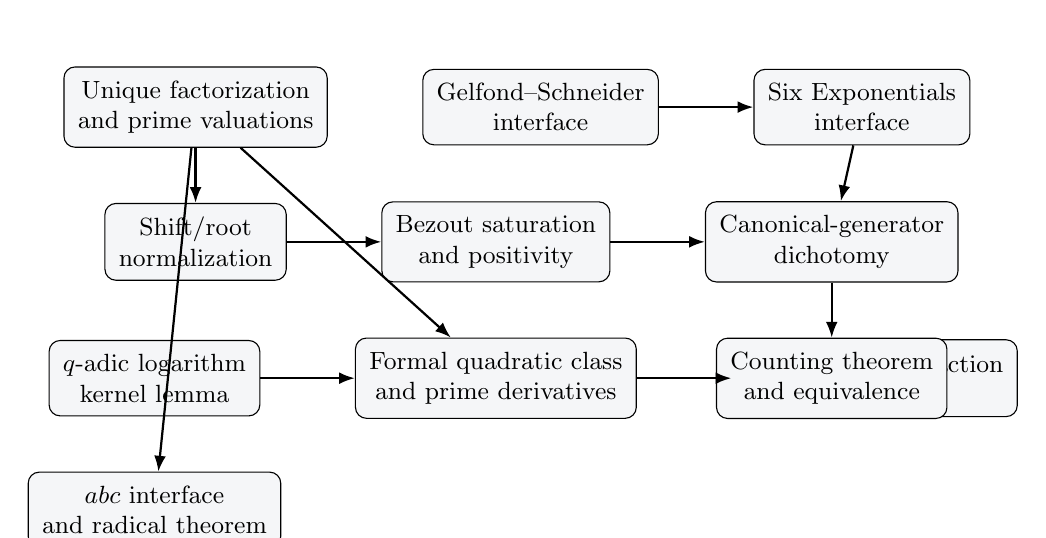
\begin{tikzpicture}[
  node distance=7mm and 12mm,
  box/.style={draw,rounded corners,align=center,fill=softgray,inner sep=5pt,font=\small},
  arr/.style={-{Latex[length=2mm]},thick}
]
\node[box] (ufd) {Unique factorization\\and prime valuations};
\node[box, right=of ufd] (gs) {Gelfond--Schneider\\interface};
\node[box, right=of gs] (six) {Six Exponentials\\interface};
\node[box, below=of ufd] (norm) {Shift/root\\normalization};
\node[box, right=of norm] (sat) {Bezout saturation\\and positivity};
\node[box, right=of sat] (dich) {Canonical-generator\\dichotomy};
\node[box, below=of sat] (quad) {Formal quadratic class\\and prime derivatives};
\node[box, left=of quad] (qadic) {$q$-adic logarithm\\kernel lemma};
\node[box, right=of quad] (period) {Sparse period/coaction\\interface};
\node[box, below=of dich] (count) {Counting theorem\\and equivalence};
\node[box, below=of qadic] (abc) {$abc$ interface\\and radical theorem};

\draw[arr] (ufd) -- (norm);
\draw[arr] (norm) -- (sat);
\draw[arr] (six) -- (dich);
\draw[arr] (sat) -- (dich);
\draw[arr] (gs) -- (six);
\draw[arr] (dich) -- (count);
\draw[arr] (ufd) -- (quad);
\draw[arr] (quad) -- (period);
\draw[arr] (qadic) -- (quad);
\draw[arr] (ufd) -- (abc);
\end{tikzpicture}
\end{center}

\subsection{What can be formalized immediately}

The following pieces require only standard algebra and real analysis infrastructure.

\begin{enumerate}
\item Prime factorization vectors for positive natural numbers.
\item The shift normalization $k=\min(v_2(m),v_3(n))$.
\item Common-perfect-power extraction by the gcd of factorization coefficients.
\item The valuation criterion for $y=(A+B\xi)/D$.
\item The Bezout denominator-elimination proof.
\item Positivity of $A,B$ from one external prime and one zero diagonal valuation.
\item Uniqueness of the normalized primitive generator, assuming the exceptional-plane statement.
\item The lattice-point count in a rational triangle with irrational slope.
\item The formal polynomial $\mathcal F_{m,n}$, its vanishing classification, and its derivatives.
\item The elementary lower bound \eqref{eq:elementarylower}.
\item The kernel calculation for $\log_q$ on positive rationals, once a standard $q$-adic logarithm API is available.
\end{enumerate}

\subsection{Interfaces for deep theorems}

A robust formal development should isolate rather than blur the non-elementary inputs.

\begin{lstlisting}
-- Schematic only; names are not asserted to match current mathlib.

axiom gelfond_schneider_real
  (a x : Real) (ha : IsAlgebraic a) (hx : IsAlgebraic x)
  (ha0 : a != 0) (ha1 : a != 1) (hxirr : x !in Rational) :
  Transcendental (Real.rpow a x)

axiom six_exponentials_dim_bound :
  finrank Rational AlgebraicExponentSpace23 <= 2

structure SparseCoactionSeparation : Prop where
  descend : forall (m n q : Nat),
    Prime q -> q != 2 -> q != 3 ->
    log m * log 3 = log n * log 2 ->
    valuation q m * log 3 = valuation q n * log 2

structure ABCConjecture : Prop where
  bound : forall epsilon > 0, exists K, ...
\end{lstlisting}

The main formal theorem can then be stated in layers:
\begin{itemize}
\item under Gelfond--Schneider and Six Exponentials, prove the canonical-generator dichotomy;
\item under sparse coaction separation, prove the conjecture;
\item under $abc$, prove radical fullness of the reduced gaps.
\end{itemize}
This gives a meaningful Lean artifact even before every transcendence input is present: the elementary reduction from each named interface to the final conclusion can be machine-checked independently.

\subsection{Suggested theorem order}

\begin{enumerate}
\item \texttt{rational\_candidate\_integer}.
\item \texttt{support\_subset\_two\_three\_forces\_integer}.
\item \texttt{normalize\_candidate}.
\item \texttt{valuation\_denominator\_divisibility}.
\item \texttt{primitive\_saturation\_denominator\_one}.
\item \texttt{all\_solutions\_eq\_nat\_span}.
\item \texttt{normalized\_primitive\_unique}.
\item \texttt{solution\_count\_quadratic}.
\item \texttt{sparse\_quad\_nonzero}.
\item \texttt{external\_derivative\_nonzero}.
\item \texttt{qadic\_mixed\_realization\_nonzero}.
\item \texttt{abc\_gap\_radical\_ratio}.
\end{enumerate}

\section{Prioritized research program}

\subsection{Priority A: exploit the canonical counting threshold}

The dichotomy converts the conjecture into a quantitative statement about integer points:
\[
  N(H)=o((\log H)^2).
\]
A promising plan is to divide the curve into logarithmic boxes, construct local interpolation determinants from integer points, and use the special self-similarity
\[
  (X,Y)\mapsto(2X,3Y)
\]
together with an external-prime filtration.  The target is not an arbitrary power saving in $H$, but only a saving over the quadratic power of $\log H$.

\paragraph{Kill criterion.}
Any method whose best upper bound remains $O((\log H)^C)$ with $C\ge2$ cannot decide the problem without additional structural input.

\subsection{Priority B: prove sparse coaction separation}

The period class is exceptionally restricted:
\[
  \ell(m)\ell(3)-\ell(n)\ell(2).
\]
Its coaction descendant at an external prime is a single rational logarithm.  Rather than attack full Schanuel or full period injectivity, one should seek a theorem for decomposable weight-two Kummer products with one fixed factor in $\{\ell2,\ell3\}$.

Possible tools include:
\begin{itemize}
\item zero estimates for the unipotent fundamental group of $\mathbb G_m\setminus S$ in weight at most two;
\item explicit comparison of archimedean and semistable $q$-adic realizations;
\item a slope inequality for the tiny Tannakian subcategory generated by the four Kummer classes $2,3,m,n$;
\item a restricted period matrix whose determinant factors through the external derivative $\Lambda_q$.
\end{itemize}

\paragraph{Kill criterion.}
An argument that uses only the numerical equality of products of logarithms, without a mechanism making the relation coaction-stable, risks silently assuming the desired period injectivity.

\subsection{Priority C: separate coaction ranks one and two}

In rank two, two external primes produce independent descendants.  This is the natural case for an adelic determinant with two finite-place gains.  In rank one, the entire external support is a common integer $U$, and one faces the special three-logarithm relation \eqref{eq:rankonerelation}.  The latter should be attacked directly, perhaps by a tailored three-variable auxiliary function rather than by a general many-prime construction.

\paragraph{Milestone C1.}
Prove the conjecture when the external exponent matrix has rank two.

\paragraph{Milestone C2.}
Prove the conjecture for the rank-one normal form
\[
 m=2^a3^cU^A,
 \qquad
 n=2^b3^dU^B.
\]
These two milestones partition all counterexamples.

\subsection{Priority D: manufacture a third algebraic exponent}

By Six Exponentials, a counterexample exhausts the entire two-dimensional algebraic-exponent space.  It is therefore enough to force one nonlinear exponent, especially $x^2$, back into that space.  Candidate mechanisms worth testing include:
\begin{itemize}
\item algebraicity of a carefully chosen special-function value that can be rewritten as both $2^{P(x)}$ and $3^{P(x)}$;
\item a functional equation on the semigroup grid that closes under multiplication of exponents rather than only addition;
\item an algebraic correspondence on $\mathbb G_m^2$ sending the one-parameter subgroup to itself with parameter $t\mapsto t^2$.
\end{itemize}
Any one of these would contradict the corollary that $x^2\notin\Espace$.

\subsection{Priority E: use $abc$ as a diagnostic, not as a presumed proof}

The radical-full theorem says that a gap-based Frey curve will generally carry a large new conductor.  Future modular experiments should therefore demonstrate an independent reason why those gap primes disappear from the residual conductor.  Without such a mechanism, increasing the exponent merely increases the level.

\section{Detailed comparison of proof obligations}

\begin{longtable}{>{\raggedright\arraybackslash}p{0.25\textwidth} >{\raggedright\arraybackslash}p{0.31\textwidth} >{\raggedright\arraybackslash}p{0.34\textwidth}}
\toprule
Route & What is already rigorous & Exact missing step\\
\midrule
\endfirsthead
\toprule
Route & What is already rigorous & Exact missing step\\
\midrule
\endhead
Six Exponentials/counting & Exceptional plane, normalized saturation, unique generator, quadratic point count & Beat the $(\log H)^2$ threshold using the special arithmetic of $\alpha=\log3/\log2$.\\
\addlinespace
Motivic coaction & Nonzero weight-two class; explicit nonzero first descendant & Infer coaction-stable vanishing from one zero archimedean period.\\
\addlinespace
$q$-adic comparison & Canonical external prime and nonzero $\log_q(3^{a_q}/2^{b_q})$ & Relate the archimedean zero to the local mixed regulator.\\
\addlinespace
Auxiliary determinants & Full two-dimensional grid of integer points & Extract independent information despite scalar collapse of the primitive period relation.\\
\addlinespace
Frey/$abc$ & Coprime gap equations; conditional radical fullness & Remove exponentially many gap primes from the lowered level, or find a different modular encoding.\\
\addlinespace
Nonlinear exponent bootstrap & $x^2$ is provably outside the algebraic-exponent plane & Prove both $2^{x^2}$ and $3^{x^2}$ algebraic from the original integrality.\\
\bottomrule
\end{longtable}

\section{Conclusions}

The work reported here does not complete an unconditional proof, but it substantially sharpens the frontier.

\begin{enumerate}
\item A counterexample is not an arbitrary isolated transcendental exponent.  After an explicit normalization it is a unique canonical generator $\xi$, and every solution is $r+s\xi$ with $r,s\ge0$.
\item Therefore one extra integer point forces an exact quadratic-logarithmic point-count asymptotic.  The conjecture is equivalent to any subquadratic-logarithmic upper bound.
\item The primitive quadratic logarithm relation is a nonzero sparse weight-two Kummer class.  Every external support prime gives a nonzero first coaction descendant and a nonzero $q$-adic mixed realization.
\item The counterexample would thus violate a very small, explicit period-separation principle, not merely an amorphous global conjecture.
\item Assuming $abc$, the natural continued-fraction gaps are radical-full.  This explains why a straightforward Frey curve does not automatically benefit from the repeated powers in the main terms.
\item The elementary and conditional components admit a clean Lean dependency architecture.  Formalization can begin immediately without pretending that the missing transcendence inputs are already available.
\end{enumerate}

The two most credible next attacks are now sharply stated: prove a sub-$(\log H)^2$ counting theorem using external-prime divisibility, or prove sparse coaction separation for the decomposable class \eqref{eq:motivicclass}.  Either result would settle the Alaoglu--Erd\H{o}s conjecture.

\appendix

\section{A Smith-normal-form version of saturation}

For completeness, let $C$ be the integer matrix with rows
\[
 (1,a_2),\quad(0,a_p)\ (p\ne2),\quad
 (1,b_3),\quad(0,b_p)\ (p\ne3),
\]
with zero rows omitted.  Define
\[
 L_C=\{z\in\Q^2:Cz\in\Z^r\}.
\]
Then $\Z^2\subseteq L_C$, and Smith normal form gives
\[
  \#(L_C/\Z^2)=\gcd\{\text{$2\times2$ minors of }C\}.
\]
The only nonzero maximal minors are, up to sign,
\[
  b_3-a_2,
  \qquad a_p\ (p\ne2),
  \qquad b_p\ (p\ne3).
\]
This yields \eqref{eq:saturation-index}.  Shift normalization identifies that gcd with the common perfect-power exponent; primitive descent makes it one.  Hence $L_C=\Z^2$.

The Bezout proof in the main text is the coordinate form of this Smith-normal-form argument.

\section{Proof of the $q$-adic logarithm kernel statement}

Let $q$ be odd.  Every $u\in\Q_q^\times$ has a unique decomposition
\[
 u=q^{v_q(u)}\omega(u)\langle u\rangle,
\]
where $\omega(u)$ is a Teichm\"uller root of unity and $\langle u\rangle\in1+q\Z_q$.  The standard logarithm kills $q$ and $\omega(u)$ and is injective on $1+q\Z_q$.  If $u\in\Q_{>0}^\times$ and $\log_qu=0$, then $\langle u\rangle=1$, so
\[
 u=q^{v_q(u)}\omega(u).
\]
The only positive rational root of unity is $1$.  Hence $u=q^k$ for some $k\in\Z$.  If additionally $v_q(u)=0$, then $u=1$.

For the external derivative ratio $R_q=3^{a_q}/2^{b_q}$, one has $v_q(R_q)=0$, and $R_q\ne1$.  Therefore $\log_qR_q\ne0$.

\section{A precise point-count calculation}

Let $\xi>0$ be irrational.  The number of pairs $(r,s)\in\N_0^2$ with
\[
 r+s\xi\le T
\]
is
\[
 \sum_{s=0}^{\lfloor T/\xi\rfloor}
 \bigl(\lfloor T-s\xi\rfloor+1\bigr).
\]
Writing $S=\lfloor T/\xi\rfloor$ and replacing each floor by its argument plus an error bounded by $1$ gives
\begin{align*}
 A(T)
 &=\sum_{s=0}^{S}(T-s\xi+1)+O(S)\\
 &=(S+1)(T+1)-\frac{\xi S(S+1)}2+O(S)\\
 &=\frac{T^2}{2\xi}+O_\xi(T).
\end{align*}
With $T=\log H/\log3$, this becomes the second asymptotic in Corollary~\ref{cor:counting}.

\section{Formal derivative identities at all primes}

For reference, the derivatives of \eqref{eq:formalF} are
\begin{align*}
 \partial_q\mathcal F_{m,n}
 &=a_qL_3-b_qL_2,
 &&q\notin\{2,3\},\\
 \partial_2\mathcal F_{m,n}
 &=a_2L_3-b_2L_2-L(n),\\
 \partial_3\mathcal F_{m,n}
 &=a_3L_3+L(m)-b_3L_2.
\end{align*}
At a candidate point, the last two evaluate to
\begin{align*}
 \operatorname{ev}_\infty(\partial_2\mathcal F)
 &=(a_2-x)\log3-b_2\log2,\\
 \operatorname{ev}_\infty(\partial_3\mathcal F)
 &=a_3\log3+(x-b_3)\log2.
\end{align*}
The external primes are special because their derivatives eliminate $x$ completely and become logarithms of explicit rational numbers.

Euler's identity for a homogeneous quadratic polynomial gives
\[
  2\mathcal F_{m,n}=\sum_q L_q\partial_q\mathcal F_{m,n}.
\]
Thus the zero period is a weighted cancellation among its first derivatives.  The external derivative theorem says at least one of those summands is unconditionally nonzero after real evaluation.

\section{References}

\begin{thebibliography}{99}

\bibitem{AE1944}
L. Alaoglu and P. Erd\H{o}s,
\emph{On highly composite and similar numbers},
Transactions of the American Mathematical Society \textbf{56} (1944), 448--469.

\bibitem{Baker1966}
A. Baker,
\emph{Linear forms in the logarithms of algebraic numbers. I--IV},
Mathematika \textbf{13--15} (1966--1968).

\bibitem{BakerBook}
A. Baker,
\emph{Transcendental Number Theory},
Cambridge University Press, 1975.

\bibitem{Bugeaud}
Y. Bugeaud,
\emph{Linear Forms in Logarithms and Applications},
IRMA Lectures in Mathematics and Theoretical Physics, European Mathematical Society, 2018.

\bibitem{Brown2012}
F. Brown,
\emph{Mixed Tate motives over $\mathbb Z$},
Annals of Mathematics \textbf{175} (2012), 949--976.

\bibitem{BrunsGubeladze}
W. Bruns and J. Gubeladze,
\emph{Polytopes, Rings, and $K$-Theory},
Springer, 2009.

\bibitem{DeligneGoncharov}
P. Deligne and A. B. Goncharov,
\emph{Groupes fondamentaux motiviques de Tate mixte},
Annales Scientifiques de l'\'Ecole Normale Sup\'erieure \textbf{38} (2005), 1--56.

\bibitem{Gelfond}
A. O. Gelfond,
\emph{Transcendental and Algebraic Numbers},
Dover, 1960.

\bibitem{HuberMullerStach}
A. Huber and S. M\"uller-Stach,
\emph{Periods and Nori Motives},
Springer, 2017.

\bibitem{KontsevichZagier}
M. Kontsevich and D. Zagier,
\emph{Periods},
in \emph{Mathematics Unlimited---2001 and Beyond}, Springer, 2001, 771--808.

\bibitem{Lang}
S. Lang,
\emph{Introduction to Transcendental Numbers},
Addison--Wesley, 1966.

\bibitem{LaurentMignotteNesterenko}
M. Laurent, M. Mignotte, and Yu. Nesterenko,
\emph{Formes lin\'eaires en deux logarithmes et d\'eterminants d'interpolation},
Journal of Number Theory \textbf{55} (1995), 285--321.

\bibitem{Matveev}
E. M. Matveev,
\emph{An explicit lower bound for a homogeneous rational linear form in logarithms of algebraic numbers. II},
Izvestiya: Mathematics \textbf{64} (2000), 1217--1269.

\bibitem{PilaWilkie}
J. Pila and A. J. Wilkie,
\emph{The rational points of a definable set},
Duke Mathematical Journal \textbf{133} (2006), 591--616.

\bibitem{WaldschmidtBook}
M. Waldschmidt,
\emph{Diophantine Approximation on Linear Algebraic Groups},
Springer, 2000.

\bibitem{WaldschmidtOpen}
M. Waldschmidt,
\emph{Open Diophantine problems},
Moscow Mathematical Journal \textbf{4} (2004), 245--305.

\end{thebibliography}

\end{document}
